%%
% Copyright (c) 2017 - 2024, Pascal Wagler;
% Copyright (c) 2014 - 2024, John MacFarlane
%
% All rights reserved.
%
% Redistribution and use in source and binary forms, with or without
% modification, are permitted provided that the following conditions
% are met:
%
% - Redistributions of source code must retain the above copyright
% notice, this list of conditions and the following disclaimer.
%
% - Redistributions in binary form must reproduce the above copyright
% notice, this list of conditions and the following disclaimer in the
% documentation and/or other materials provided with the distribution.
%
% - Neither the name of John MacFarlane nor the names of other
% contributors may be used to endorse or promote products derived
% from this software without specific prior written permission.
%
% THIS SOFTWARE IS PROVIDED BY THE COPYRIGHT HOLDERS AND CONTRIBUTORS
% "AS IS" AND ANY EXPRESS OR IMPLIED WARRANTIES, INCLUDING, BUT NOT
% LIMITED TO, THE IMPLIED WARRANTIES OF MERCHANTABILITY AND FITNESS
% FOR A PARTICULAR PURPOSE ARE DISCLAIMED. IN NO EVENT SHALL THE
% COPYRIGHT OWNER OR CONTRIBUTORS BE LIABLE FOR ANY DIRECT, INDIRECT,
% INCIDENTAL, SPECIAL, EXEMPLARY, OR CONSEQUENTIAL DAMAGES (INCLUDING,
% BUT NOT LIMITED TO, PROCUREMENT OF SUBSTITUTE GOODS OR SERVICES;
% LOSS OF USE, DATA, OR PROFITS; OR BUSINESS INTERRUPTION) HOWEVER
% CAUSED AND ON ANY THEORY OF LIABILITY, WHETHER IN CONTRACT, STRICT
% LIABILITY, OR TORT (INCLUDING NEGLIGENCE OR OTHERWISE) ARISING IN
% ANY WAY OUT OF THE USE OF THIS SOFTWARE, EVEN IF ADVISED OF THE
% POSSIBILITY OF SUCH DAMAGE.
%%

%%
% This is the Eisvogel pandoc LaTeX template.
%
% For usage information and examples visit the official GitHub page:
% https://github.com/Wandmalfarbe/pandoc-latex-template
%%

% Options for packages loaded elsewhere
\PassOptionsToPackage{unicode}{hyperref}
\PassOptionsToPackage{hyphens}{url}
\PassOptionsToPackage{dvipsnames,svgnames,x11names,table}{xcolor}
%
\documentclass[
  paper=a4,
  ,captions=tableheading
]{scrartcl}
\usepackage{amsmath,amssymb}
% Use setspace anyway because we change the default line spacing.
% The spacing is changed early to affect the titlepage and the TOC.
\usepackage{setspace}
\setstretch{1.2}
\usepackage{iftex}
\ifPDFTeX
  \usepackage[T1]{fontenc}
  \usepackage[utf8]{inputenc}
  \usepackage{textcomp} % provide euro and other symbols
\else % if luatex or xetex
  \usepackage{unicode-math} % this also loads fontspec
  \defaultfontfeatures{Scale=MatchLowercase}
  \defaultfontfeatures[\rmfamily]{Ligatures=TeX,Scale=1}
\fi
\usepackage{lmodern}
\ifPDFTeX\else
  % xetex/luatex font selection
\fi
% Use upquote if available, for straight quotes in verbatim environments
\IfFileExists{upquote.sty}{\usepackage{upquote}}{}
\IfFileExists{microtype.sty}{% use microtype if available
  \usepackage[]{microtype}
  \UseMicrotypeSet[protrusion]{basicmath} % disable protrusion for tt fonts
}{}
\makeatletter
\@ifundefined{KOMAClassName}{% if non-KOMA class
  \IfFileExists{parskip.sty}{%
    \usepackage{parskip}
  }{% else
    \setlength{\parindent}{0pt}
    \setlength{\parskip}{6pt plus 2pt minus 1pt}}
}{% if KOMA class
  \KOMAoptions{parskip=half}}
\makeatother
\usepackage{xcolor}
\definecolor{default-linkcolor}{HTML}{A50000}
\definecolor{default-filecolor}{HTML}{A50000}
\definecolor{default-citecolor}{HTML}{4077C0}
\definecolor{default-urlcolor}{HTML}{4077C0}
\usepackage[top=1in,bottom=1in]{geometry}
\usepackage{longtable,booktabs,array}
\usepackage{calc} % for calculating minipage widths
% Correct order of tables after \paragraph or \subparagraph
\usepackage{etoolbox}
\makeatletter
\patchcmd\longtable{\par}{\if@noskipsec\mbox{}\fi\par}{}{}
\makeatother
% Allow footnotes in longtable head/foot
\IfFileExists{footnotehyper.sty}{\usepackage{footnotehyper}}{\usepackage{footnote}}
\makesavenoteenv{longtable}
% add backlinks to footnote references, cf. https://tex.stackexchange.com/questions/302266/make-footnote-clickable-both-ways
\usepackage{footnotebackref}
\usepackage{graphicx}
\makeatletter
\newsavebox\pandoc@box
\newcommand*\pandocbounded[1]{% scales image to fit in text height/width
  \sbox\pandoc@box{#1}%
  \Gscale@div\@tempa{\textheight}{\dimexpr\ht\pandoc@box+\dp\pandoc@box\relax}%
  \Gscale@div\@tempb{\linewidth}{\wd\pandoc@box}%
  \ifdim\@tempb\p@<\@tempa\p@\let\@tempa\@tempb\fi% select the smaller of both
  \ifdim\@tempa\p@<\p@\scalebox{\@tempa}{\usebox\pandoc@box}%
  \else\usebox{\pandoc@box}%
  \fi%
}
% Set default figure placement to htbp
% Make use of float-package and set default placement for figures to H.
% The option H means 'PUT IT HERE' (as  opposed to the standard h option which means 'You may put it here if you like').
\usepackage{float}
\floatplacement{figure}{H}
\makeatother
\setlength{\emergencystretch}{3em} % prevent overfull lines
\providecommand{\tightlist}{%
  \setlength{\itemsep}{0pt}\setlength{\parskip}{0pt}}
\setcounter{secnumdepth}{-\maxdimen} % remove section numbering
\ifLuaTeX
\usepackage[bidi=basic]{babel}
\else
\usepackage[bidi=default]{babel}
\fi
\babelprovide[main,import]{english}
% get rid of language-specific shorthands (see #6817):
\let\LanguageShortHands\languageshorthands
\def\languageshorthands#1{}
\makeatletter
\@ifpackageloaded{subfig}{}{\usepackage{subfig}}
\@ifpackageloaded{caption}{}{\usepackage{caption}}
\captionsetup[subfloat]{margin=0.5em}
\AtBeginDocument{%
\renewcommand*\figurename{Figura}
\renewcommand*\tablename{Tabla}
}
\AtBeginDocument{%
\renewcommand*\listfigurename{Lista de Figuras}
\renewcommand*\listtablename{Lista de Tablas}
}
\newcounter{pandoccrossref@subfigures@footnote@counter}
\newenvironment{pandoccrossrefsubfigures}{%
\setcounter{pandoccrossref@subfigures@footnote@counter}{0}
\begin{figure}\centering%
\gdef\global@pandoccrossref@subfigures@footnotes{}%
\DeclareRobustCommand{\footnote}[1]{\footnotemark%
\stepcounter{pandoccrossref@subfigures@footnote@counter}%
\ifx\global@pandoccrossref@subfigures@footnotes\empty%
\gdef\global@pandoccrossref@subfigures@footnotes{{##1}}%
\else%
\g@addto@macro\global@pandoccrossref@subfigures@footnotes{, {##1}}%
\fi}}%
{\end{figure}%
\addtocounter{footnote}{-\value{pandoccrossref@subfigures@footnote@counter}}
\@for\f:=\global@pandoccrossref@subfigures@footnotes\do{\stepcounter{footnote}\footnotetext{\f}}%
\gdef\global@pandoccrossref@subfigures@footnotes{}}
\@ifpackageloaded{float}{}{\usepackage{float}}
\floatstyle{ruled}
\@ifundefined{c@chapter}{\newfloat{codelisting}{h}{lop}}{\newfloat{codelisting}{h}{lop}[chapter]}
\floatname{codelisting}{Listing}
\newcommand*\listoflistings{\listof{codelisting}{Listas del Documento}}
\makeatother
\usepackage{bookmark}
\IfFileExists{xurl.sty}{\usepackage{xurl}}{} % add URL line breaks if available
\urlstyle{same}
\hypersetup{
  pdftitle={Documento de Especificación de Entregas},
  pdflang={en},
  pdfsubject={Implementación Proyecto},
  pdfkeywords={Integración, Interoperabilidad, JEP, Softgic},
  hidelinks,
  breaklinks=true,
  pdfcreator={LaTeX via pandoc with the Eisvogel template}}
\title{Documento de Especificación de Entregas}
\usepackage{etoolbox}
\makeatletter
\providecommand{\subtitle}[1]{% add subtitle to \maketitle
  \apptocmd{\@title}{\par {\large #1 \par}}{}{}
}
\makeatother
\subtitle{Implementación Proyecto Evolución de Interoperabilidad JEP,
Softgic}
\author{}
\date{2024-09-16}



%%
%% added
%%


%
% for the background color of the title page
%
\usepackage{pagecolor}
\usepackage{afterpage}
\usepackage{tikz}

%
% break urls
%
\PassOptionsToPackage{hyphens}{url}

%
% When using babel or polyglossia with biblatex, loading csquotes is recommended
% to ensure that quoted texts are typeset according to the rules of your main language.
%
\usepackage{csquotes}

%
% captions
%
\definecolor{caption-color}{HTML}{777777}
\usepackage[font={stretch=1.2}, textfont={color=caption-color}, position=top, skip=4mm, labelfont=bf, singlelinecheck=false, justification=raggedright]{caption}
\setcapindent{0em}

%
% blockquote
%
\definecolor{blockquote-border}{RGB}{221,221,221}
\definecolor{blockquote-text}{RGB}{119,119,119}
\usepackage{mdframed}
\newmdenv[rightline=false,bottomline=false,topline=false,linewidth=3pt,linecolor=blockquote-border,skipabove=\parskip]{customblockquote}
\renewenvironment{quote}{\begin{customblockquote}\list{}{\rightmargin=0em\leftmargin=0em}%
\item\relax\color{blockquote-text}\ignorespaces}{\unskip\unskip\endlist\end{customblockquote}}

%
% Source Sans Pro as the default font family
% Source Code Pro for monospace text
%
% 'default' option sets the default
% font family to Source Sans Pro, not \sfdefault.
%
\ifnum 0\ifxetex 1\fi\ifluatex 1\fi=0 % if pdftex
    \usepackage[default]{sourcesanspro}
  \usepackage{sourcecodepro}
  \else % if not pdftex
    \usepackage[default]{sourcesanspro}
  \usepackage{sourcecodepro}

  % XeLaTeX specific adjustments for straight quotes: https://tex.stackexchange.com/a/354887
  % This issue is already fixed (see https://github.com/silkeh/latex-sourcecodepro/pull/5) but the
  % fix is still unreleased.
  % TODO: Remove this workaround when the new version of sourcecodepro is released on CTAN.
  \ifxetex
    \makeatletter
    \defaultfontfeatures[\ttfamily]
      { Numbers   = \sourcecodepro@figurestyle,
        Scale     = \SourceCodePro@scale,
        Extension = .otf }
    \setmonofont
      [ UprightFont    = *-\sourcecodepro@regstyle,
        ItalicFont     = *-\sourcecodepro@regstyle It,
        BoldFont       = *-\sourcecodepro@boldstyle,
        BoldItalicFont = *-\sourcecodepro@boldstyle It ]
      {SourceCodePro}
    \makeatother
  \fi
  \fi

%
% heading color
%
\definecolor{heading-color}{RGB}{40,40,40}
\addtokomafont{section}{\color{heading-color}}
% When using the classes report, scrreprt, book,
% scrbook or memoir, uncomment the following line.
%\addtokomafont{chapter}{\color{heading-color}}

%
% variables for title, author and date
%
\usepackage{titling}
\title{Documento de Especificación de Entregas}
\author{}
\date{2024-09-16}

%
% tables
%

\definecolor{table-row-color}{HTML}{F5F5F5}
\definecolor{table-rule-color}{HTML}{999999}

%\arrayrulecolor{black!40}
\arrayrulecolor{table-rule-color}     % color of \toprule, \midrule, \bottomrule
\setlength\heavyrulewidth{0.3ex}      % thickness of \toprule, \bottomrule
\renewcommand{\arraystretch}{1.3}     % spacing (padding)


%
% remove paragraph indentation
%
\setlength{\parindent}{0pt}
\setlength{\parskip}{6pt plus 2pt minus 1pt}
\setlength{\emergencystretch}{3em}  % prevent overfull lines

%
%
% Listings
%
%


%
% header and footer
%
\usepackage[headsepline,footsepline]{scrlayer-scrpage}

\newpairofpagestyles{eisvogel-header-footer}{
  \clearpairofpagestyles
  \ihead*{
\includegraphics{include/jeplogo.jpg}}
  \chead*{}
  \ohead*{2024-09-16}
  \ifoot*{}
  \cfoot*{}
  \ofoot*{\thepage}
  \addtokomafont{pageheadfoot}{\upshape}
}
\pagestyle{eisvogel-header-footer}



%%
%% end added
%%

\begin{document}

%%
%% begin titlepage
%%
\begin{titlepage}
\newgeometry{top=2cm, right=4cm, bottom=3cm, left=4cm}
\tikz[remember picture,overlay] \node[inner sep=0pt] at (current page.center){
\includegraphics[width=\paperwidth,height=\paperheight]{include/softgicbackgr.png}};
\newcommand{\colorRule}[3][black]{\textcolor[HTML]{#1}{\rule{#2}{#3}}}
\begin{flushleft}
\noindent
\\[-1em]
\color[HTML]{5F5F5F}
\makebox[0pt][l]{\colorRule[360049]{1.3\textwidth}{4pt}}
\par
\noindent

% The titlepage with a background image has other text spacing and text size
{
  \setstretch{2}
  \vfill
  \vskip -8em
  \noindent {\huge \textbf{\textsf{Documento de Especificación de
Entregas}}}
    \vskip 1em
  {\Large \textsf{Implementación Proyecto Evolución de Interoperabilidad
JEP, Softgic}}
    \vskip 2em
  \noindent {\Large \textsf{} \vskip 0.6em \textsf{2024-09-16}}
  \vfill
}


\end{flushleft}
\end{titlepage}
\restoregeometry
\pagenumbering{arabic}

%%
%% end titlepage
%%

% \maketitle


\section{Contenido}\label{sec:contenido}

\begin{itemize}
\tightlist
\item
  \hyperref[informaciuxf3n-del-documento]{Información del Documento}
\item
  \hyperref[gestiuxf3n-de-trabajo-y-requerimientos-de-interoperabilidad]{Gestión
  de Trabajo y Requerimientos de Interoperabilidad}
\item
  \hyperref[modelo-de-requerimientos-de-interoperabilidad-proyecto-jep]{Modelo
  de Requerimientos de Interoperabilidad Proyecto JEP}
\item
  \hyperref[modelo-de-despliegue-de-requerimientos-de-interoperabilidad-proyecto-jep]{Modelo
  de Despliegue de Requerimientos de Interoperabilidad Proyecto JEP}
\end{itemize}

\newpage

\section{Información del
Documento}\label{sec:informaciuxf3n-del-documento}

\subsection{Versión del Documento}\label{sec:versiuxf3n-del-documento}

\begin{quote}
\end{quote}

Versión actual: 1.23e180b - clean - Wed, 30 Oct 2024 21:45:40 -0500

Versiones Anteriores

1.23e180b - clean - Wed, 30 Oct 2024 21:45:40 -0500

\subsubsection{Realizado Por}\label{sec:realizado-por}

Sofgic.co

\subsubsection{Revisado Por}\label{sec:revisado-por}

Sofgic.co

\newpage

\section{Gestión de Trabajo y Requerimientos de
Interoperabilidad}\label{sec:gestiuxf3n-de-trabajo-y-requerimientos-de-interoperabilidad}

\subsection{Modelo de Gestión de Requerimientos de
Integración}\label{sec:modelo-de-gestiuxf3n-de-requerimientos-de-integraciuxf3n}

\begin{quote}
Modelo de Implementación Proyecto JEP, 2024. Softgic. Propuesta modelo
de gestión y atención requerimientos de integración del proyecto de
servicios de integración JEP. Ver 0.1.37
\end{quote}

El ciclo de entrega de requerimientos inicia con la planeación macro de
los objetivos entregables del proyecto de integración organizados en el
tiempo (de septiembre a diciembre del 2024).

Los roles técnicos convierten estos objetivos macro en requerimientos
comprendidos por épicas, características e historias (o casos de uso) de
integración.

Los ingenieros convierten a su vez las historias en tareas entregables,
individuales y autónomas, de tipo tarea (UT), diseño (DIS), pruebas de
calidad (QA), análisis (AN), entrega continua (CI/CD), etc. Una vez los
ingenieros tengan esta división de trabajo en tareas pueden pasar a la
implementación mediante iteraciones (ver Modelo de Implementación del
Proyecto JEP).

Los requerimientos del proyecto JEP son procesados mediante el modelo de
producción descrito más adelante.

\begin{figure}
\centering
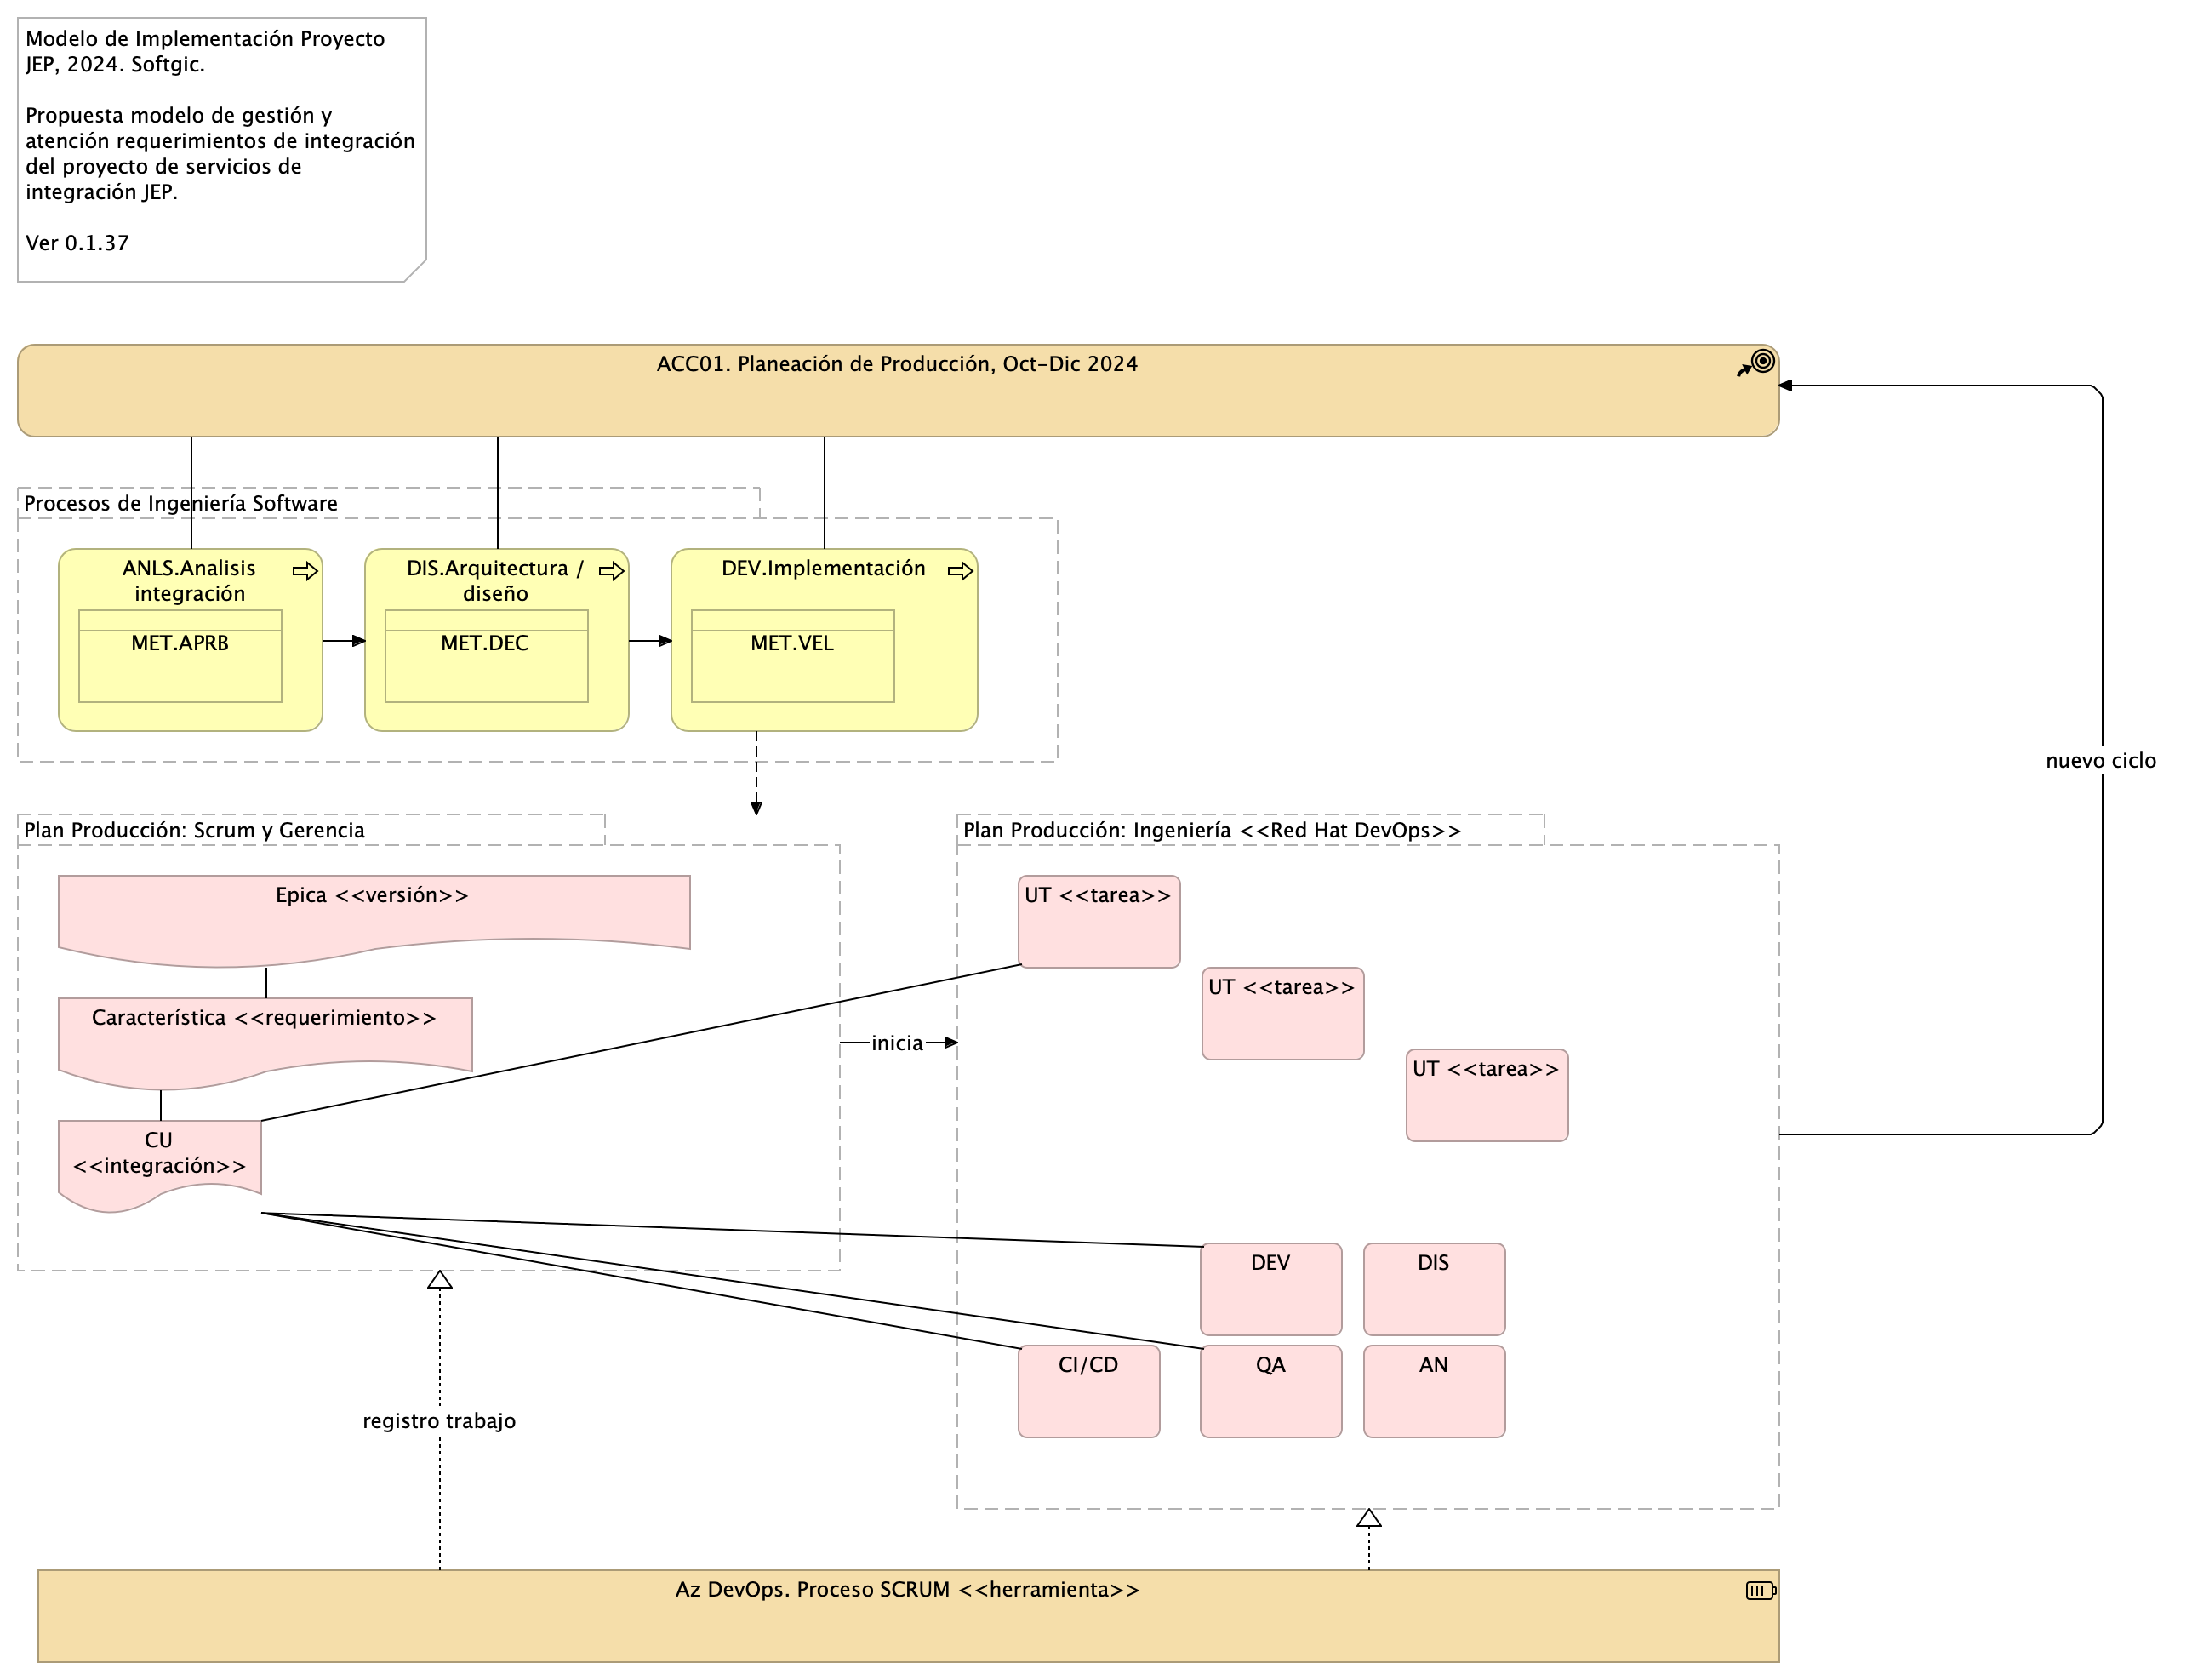
\includegraphics[width=\textwidth,height=5.20833in]{images/04.ING.2n.1a.Modelorequerimientos.png}
\caption{04.ING.2n.1a. Modelo requerimientos. \emph{Fuente: Repositorio
arquitectura Integración JEP
(2024)}}\label{fig:id-7c3abdaa8d9b46eebfd8f8e3e8d912ce}
\end{figure}

\subsubsection{Catálogo de
Elementos}\label{sec:catuxe1logo-de-elementos}

\begin{itemize}
\tightlist
\item
  \textbf{ACC01. Planeación de Producción, Oct-Dic 2024}. Objetivos y
  entregas en el tiempo, versiones de entrega del proyecto de
  integración.
\item
  \textbf{ANLS.Analisis integración}. \#\#\# 2. ANSS (análisis). *
  Scrum, Funcional, Dueño producto cliente (requiere conocimiento del
  negocio). * Resultado: Refinamiento HU, modelo de negocio, es decir,
  diagrama de HU relacionadas unas con otras y con los conceptos de
  negocio en el repositorio de ARQ. Actualmente: no hay resultados de
  este proceso. Ejemplo del modelo de negocio \#\#\# Salidas * Modelo de
  negocio en el repo * Estimación --puede en devops * Análisis de
  dependencia en el repo \#\#\# KPI - Tasa de aprobación de HU por
  cliente Fuente: (Cantidad de HU refinadas y aprobadas por cliente
  {[}Repo Sharepoint{]} / Total de cantidad de HU {[}Azure DevOps{]})
  Dato 26/10/2023: (30/44) = 0,68 - Tasa de error en Bug por PR
  entregados Fuente: (Cantidad de solicitude de cambio en rama (Pull
  Reqst) de Correcciones (fix) o Regresión (reverts) {[}Bitbucket{]} /
  Cantidad total de PR desplegados {[}Bitbucket{]}) Dato 26/10/2023:
  (8/111)*100 = 7,2\%
\item
  \textbf{CI/CD}. Actividades DevOps del ciclo o iteración de
  implementación.
\item
  \textbf{DEV}. Alcance de QA unitaria
\item
  \textbf{DEV.Implementación}. \#\#\# KPI - Velocidad de construcción
  Fuente: (Cantidad de puntos de HU ejecutadas {[}Azure DevOps{]} /
  Horas habiles del mes de trabajo {[}Calculo manual{]}) Dato
  26/10/2023: 83 / 153 = 0,54 HU/horas - Tasa de cierre de defectos
  Fuente: (Cantidad de Bug solucionados {[}Azure DevOps{]} / Total de
  Bugs a corte sin nuevos {[}Azure DevOps{]}) Dato 26/10/2023: 81 / 920
  = 0,088 - Indice de dependecia de Lider Técnico Fuente: (Cantidad de
  actividades retrazadas semanales segun las HU planeadas / Total de HU
  planeadas para ejecución) Dato 26/10/2023: Pendiente proxima semana
\item
  \textbf{DIS.Arquitectura / diseño}. \#\#\# KPI - Nivel de HU sin
  detalle técnico Fuente: (Cantidad de HU refinadas y aprobadas sin
  diseño de implementacion {[}Repo Sharepoint{]} / Total de cantidad de
  HU {[}Azure DevOps{]}) Dato 26/10/2023: 0/44=0
\item
  \textbf{MET.APRB}. Cod. APRB Nombre indicador Tasa de aprobación de HU
  por cliente Uso Estabildad de requerimientos. Contensión del flujo de
  trabajo inicio de desarrolo Proceso ANLS Calculo de medición Cantidad
  de HU refinadas y aprobadas por cliente / Total de cantidad de HU
  Fuente {[}Repo Sharepoint{]}, {[}Azure DevOps{]})
\item
  \textbf{MET.DEC}. Cod.: DEC Nombre indicador: Decisiones de diseño,
  justificaciones, validaciones Uso: Estabildad de requerimientos.
  Control de alineación desarrollo-demanda Proceso: DIS Calculo de
  medición: Cantidad de HU refinadas y aprobadas por cliente / Total de
  cantidad de HU Fuente: {[}Repo Sharepoint{]}, {[}Azure DevOps{]})\\
\item
  \textbf{MET.VEL}. Cod. VEL Nombre indicador Velocidad de construcción
  Uso Capacidad interna de desarrollo Proceso DEV Calculo de medición
  Cantidad de puntos de HU ejecutadas / Horas habiles del mes de trabajo
  Fuente {[}Azure DevOps{]}, {[}Calculo manual{]}
\item
  \textbf{UT (tarea)}. Unidad mínima de trabajo (tarea por
  desarrollador).
\end{itemize}

\subsection{Modelo de Producción e Implementación de Integración
JEP}\label{sec:modelo-de-producciuxf3n-e-implementaciuxf3n-de-integraciuxf3n-jep}

\begin{quote}
Modelo de Producción e Implementación Proyecto JEP, 2024. Softgic.
Modelo de gestión y atención requerimientos de integración del proyecto
de integración JEP, 2024. Softgic. Relación con herramienta de gestión
Az DevOps. Ver 0.1.12
\end{quote}

El modelo de producción que procesa los requerimientos del proyecto JEP
inicia con la creación de un tramo de la planeación de la solución de
integración, esto es un ciclo de implementación o iteración del proyecto
de integración JEP.

(ING) Procesos de ingeniería. Arrancan los procesos mínimos de
ingeniería previos a la construcción de la integración.

(PRY) Planificación de historias de usuario. La porción de la planeación
de producción aprobada para la construcción se planifica en historias o
casos de uso, u cualquier otra forma de medición de avance.

(ING) Creación e inicio de iteraciones de implementción incremental. La
planificación de HU (CU, u otra) es tareificada y asignada a
desarrolladores disponibles. Además, las tareas asignadas son
organizadas en ciclos de trabajo fijo (iteraciones). Esta ejecución es
la línea de trabajo principal del proyecto JEP.

(PRY, ING) Coordinación de líneas de trabajo. Las entregas de la línea
de trabajo del proyecto JEP debe ser compasada con otras líneas de
trabajo de la JEP, con las que puede haber una relación de secuencia o
dependencia externa.

Durante la ejecución de la iteraciones determinadas, inicia nuevamente
el ciclo del proyecto desde la creación de un nuevo tramo de la
planeación de producción.

\subsubsection{Mapeo del Modelo con Herramienta de Registro del Trabajo
(az
devops)}\label{sec:mapeo-del-modelo-con-herramienta-de-registro-del-trabajo-az-devops}

\begin{itemize}
\tightlist
\item
  Épica = Versión de entrega de la solución como un todo
\item
  Característica = Requerimiento de integración, del cual pueden
  desprenderse varias integraciones puntuales.
\item
  HU = Una integración puntual proveniente de un requerimiento, ej.:
  ingreso Conti, Consulta campos, Radicar ítem, Generación
  documentos\ldots{}
\item
  UT = Tarea de desarrollo.
\end{itemize}

\begin{figure}
\centering
\includegraphics[width=\textwidth,height=5.20833in]{images/04.ING.2n.1b.Modeloproducción.png}
\caption{04.ING.2n.1b. Modelo producción. \emph{Fuente: Repositorio
arquitectura Integración JEP
(2024)}}\label{fig:id-9938d5859d53450fa5c5c953d9ce33cb}
\end{figure}

\subsubsection{Catálogo de
Elementos}\label{sec:catuxe1logo-de-elementos-1}

\begin{longtable}[]{@{}
  >{\raggedright\arraybackslash}p{(\columnwidth - 4\tabcolsep) * \real{0.3000}}
  >{\raggedright\arraybackslash}p{(\columnwidth - 4\tabcolsep) * \real{0.2000}}
  >{\raggedright\arraybackslash}p{(\columnwidth - 4\tabcolsep) * \real{0.5000}}@{}}
\caption{\label{tbl:tblelement-04.ING.2n.1b.Modeloproducciuxf3n-id}Elementos
de la vista.}\tabularnewline
\toprule\noalign{}
\begin{minipage}[b]{\linewidth}\raggedright
Nombre
\end{minipage} & \begin{minipage}[b]{\linewidth}\raggedright
Tipo
\end{minipage} & \begin{minipage}[b]{\linewidth}\raggedright
Documentación
\end{minipage} \\
\midrule\noalign{}
\endfirsthead
\toprule\noalign{}
\begin{minipage}[b]{\linewidth}\raggedright
Nombre
\end{minipage} & \begin{minipage}[b]{\linewidth}\raggedright
Tipo
\end{minipage} & \begin{minipage}[b]{\linewidth}\raggedright
Documentación
\end{minipage} \\
\midrule\noalign{}
\endhead
\bottomrule\noalign{}
\endlastfoot
ACC01. Planeación de Producción, Oct-Dic 2024 & Course Of-Action &
Objetivos y entregas en el tiempo, versiones de entrega del proyecto de
integración. \\
ANLS.Analisis integración & Business Process & \#\#\# 2. ANSS
(análisis). * Scrum, Funcional, Dueño producto cliente (requiere
conocimiento del negocio). * Resultado: Refinamiento HU, modelo de
negocio, es decir, diagrama de HU relacionadas unas con otras y con los
conceptos de negocio en el repositorio de ARQ. Actualmente: no hay
resultados de este proceso. Ejemplo del modelo de negocio \#\#\# Salidas
* Modelo de negocio en el repo * Estimación --puede en devops * Análisis
de dependencia en el repo \#\#\# KPI - Tasa de aprobación de HU por
cliente Fuente: (Cantidad de HU refinadas y aprobadas por cliente
{[}Repo Sharepoint{]} / Total de cantidad de HU {[}Azure DevOps{]}) Dato
26/10/2023: (30/44) = 0,68 - Tasa de error en Bug por PR entregados
Fuente: (Cantidad de solicitude de cambio en rama (Pull Reqst) de
Correcciones (fix) o Regresión (reverts) {[}Bitbucket{]} / Cantidad
total de PR desplegados {[}Bitbucket{]}) Dato 26/10/2023: (8/111)*100 =
7,2\% \\
CI/CD & Work Package & Actividades DevOps del ciclo o iteración de
implementación. \\
DEV & Work Package & Alcance de QA unitaria \\
DEV & Work Package & Alcance de QA unitaria \\
DEV.Implementación & Business Process & \#\#\# KPI - Velocidad de
construcción Fuente: (Cantidad de puntos de HU ejecutadas {[}Azure
DevOps{]} / Horas habiles del mes de trabajo {[}Calculo manual{]}) Dato
26/10/2023: 83 / 153 = 0,54 HU/horas - Tasa de cierre de defectos
Fuente: (Cantidad de Bug solucionados {[}Azure DevOps{]} / Total de Bugs
a corte sin nuevos {[}Azure DevOps{]}) Dato 26/10/2023: 81 / 920 = 0,088
- Indice de dependecia de Lider Técnico Fuente: (Cantidad de actividades
retrazadas semanales segun las HU planeadas / Total de HU planeadas para
ejecución) Dato 26/10/2023: Pendiente proxima semana \\
DIS.Arquitectura / diseño & Business Process & \#\#\# KPI - Nivel de HU
sin detalle técnico Fuente: (Cantidad de HU refinadas y aprobadas sin
diseño de implementacion {[}Repo Sharepoint{]} / Total de cantidad de HU
{[}Azure DevOps{]}) Dato 26/10/2023: 0/44=0 \\
MET.APRB & Business Object & Cod. APRB Nombre indicador Tasa de
aprobación de HU por cliente Uso Estabildad de requerimientos.
Contensión del flujo de trabajo inicio de desarrolo Proceso ANLS Calculo
de medición Cantidad de HU refinadas y aprobadas por cliente / Total de
cantidad de HU Fuente {[}Repo Sharepoint{]}, {[}Azure DevOps{]}) \\
MET.DEC & Business Object & Cod.: DEC Nombre indicador: Decisiones de
diseño, justificaciones, validaciones Uso: Estabildad de requerimientos.
Control de alineación desarrollo-demanda Proceso: DIS Calculo de
medición: Cantidad de HU refinadas y aprobadas por cliente / Total de
cantidad de HU Fuente: {[}Repo Sharepoint{]}, {[}Azure DevOps{]}) \\
MET.VEL & Business Object & Cod. VEL Nombre indicador Velocidad de
construcción Uso Capacidad interna de desarrollo Proceso DEV Calculo de
medición Cantidad de puntos de HU ejecutadas / Horas habiles del mes de
trabajo Fuente {[}Azure DevOps{]}, {[}Calculo manual{]} \\
UT (tarea) & Work Package & Unidad mínima de trabajo (tarea por
desarrollador). \\
\end{longtable}

\newpage

\section{Modelo de Requerimientos de Interoperabilidad Proyecto
JEP}\label{sec:modelo-de-requerimientos-de-interoperabilidad-proyecto-jep}

\subsection{Requerimientos de Integración
JEP}\label{sec:requerimientos-de-integraciuxf3n-jep}

\begin{quote}
Modelo de Requerimientos Proyecto Integración JEP, 2024. Softgic.
Requerimientos, condiciones técnicas, solución del proyecto Integración
JEP, 2024. Versión 0.1.43
\end{quote}

Documentación de requerimientos del proyecto de integración JEP, 2024.
Implementados mediante el modelo de producción del proyecto.

Para la implementación de los ítems relacionados en el Anexo Nro. 1.1 --
Anexo técnico evolución plataforma de interoperabilidad -- Ficha Técnica
la hoja ``Categorías de Cotización'' contiene las necesidades a
contratar en el ámbito de la evolución tecnológica del modelo de
interoperabilidad y los desarrollos de interoperabilidad tanto con
sistemas internos, como con entidades externas. En la hoja ``Estándares
Desarrollo y Producto'' del archivo mencionado se indican los estándares
recomendados por el fabricante, para tener en cuenta en la entrega de
los servicios que se cotizan.

El Anexo Nro. 1.2 -- Acuerdos de Niveles de Servicio, explica el
procedimiento con el que se dará atención a consultas o solución de
incidencias, tanto en los sistemas operativos, como en los servicios de
interoperabilidad existentes en la actualidad y aquellos que se
contratarán en este proceso, en el sistema Bus de Interoperabilidad
implementado en la Jurisdicción Especial para la Paz.

-- Documento: Justificativo de la Contratación Invitación Pública

\begin{figure}
\centering
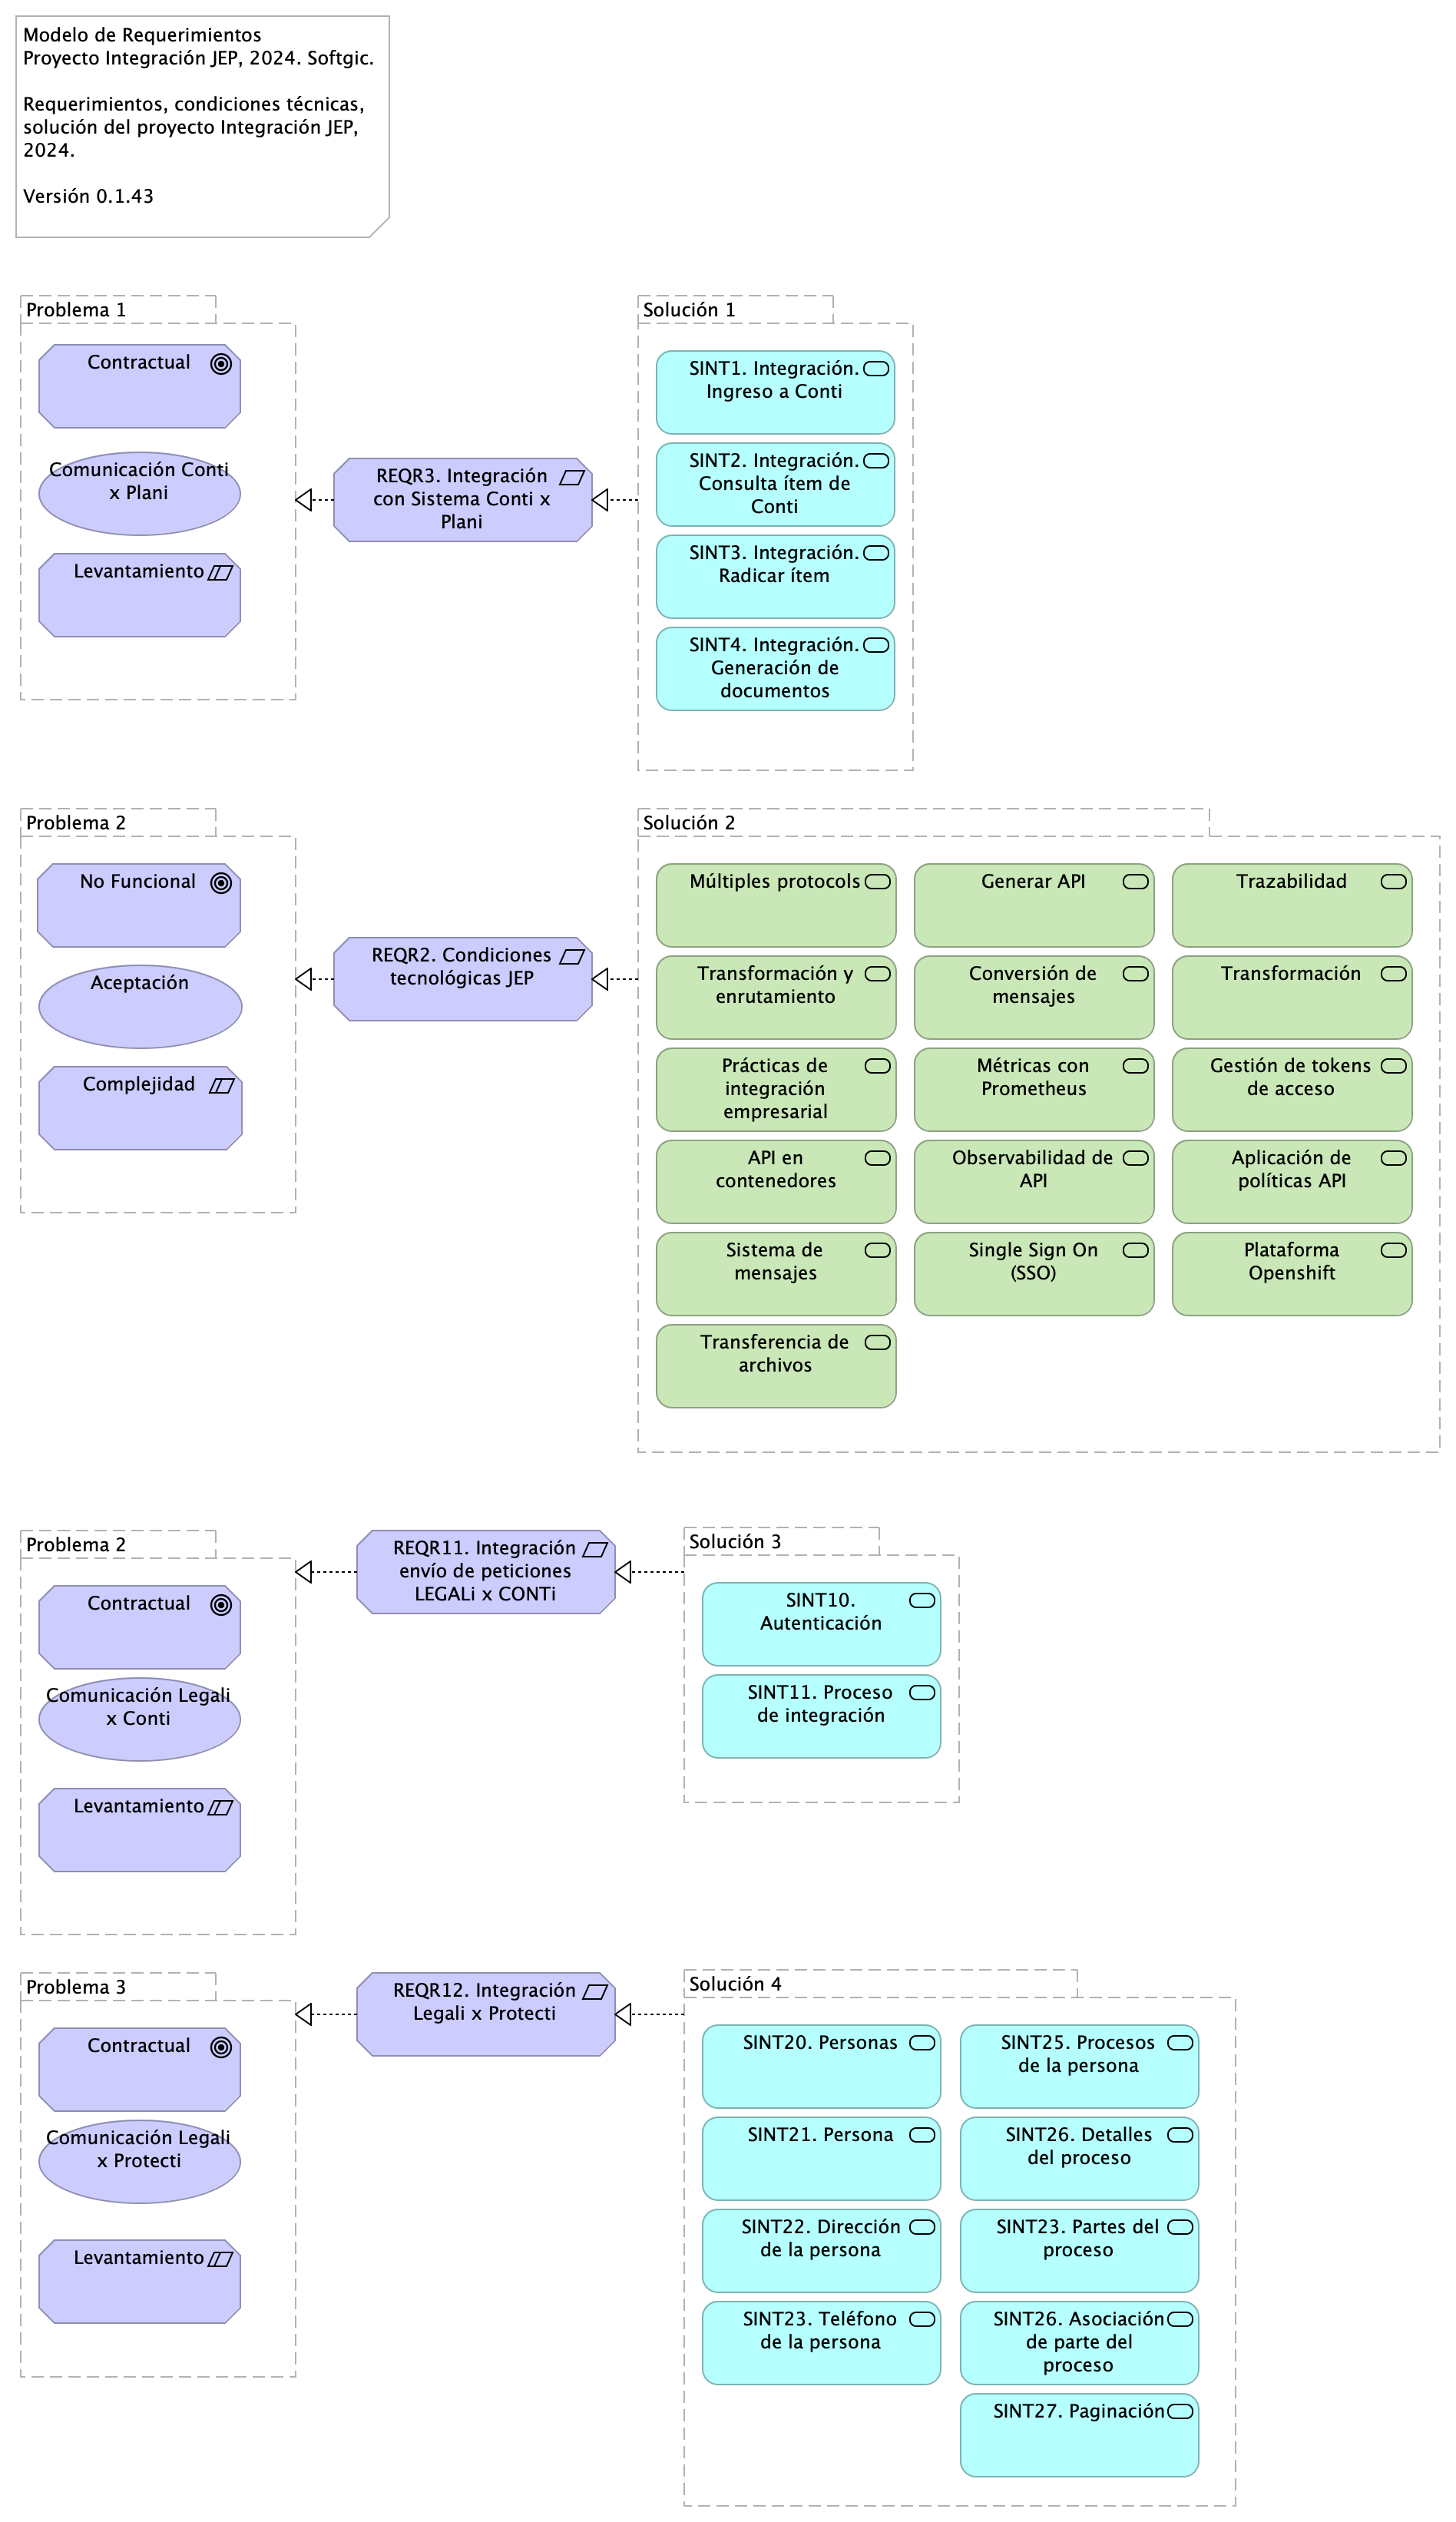
\includegraphics[width=\textwidth,height=5.20833in]{images/05.REQR.1n.Requerimientos.png}
\caption{05.REQR.1n. Requerimientos. \emph{Fuente: Repositorio
arquitectura Integración JEP
(2024)}}\label{fig:id-062616daaa1d4d8990681b58bc54ce3d}
\end{figure}

\subsubsection{Catálogo de
Elementos}\label{sec:catuxe1logo-de-elementos-2}

\begin{longtable}[]{@{}
  >{\raggedright\arraybackslash}p{(\columnwidth - 4\tabcolsep) * \real{0.3000}}
  >{\raggedright\arraybackslash}p{(\columnwidth - 4\tabcolsep) * \real{0.2000}}
  >{\raggedright\arraybackslash}p{(\columnwidth - 4\tabcolsep) * \real{0.5000}}@{}}
\caption{\label{tbl:tblelement-05.REQR.1n.Requerimientos-id}Elementos de
la vista.}\tabularnewline
\toprule\noalign{}
\begin{minipage}[b]{\linewidth}\raggedright
Nombre
\end{minipage} & \begin{minipage}[b]{\linewidth}\raggedright
Tipo
\end{minipage} & \begin{minipage}[b]{\linewidth}\raggedright
Documentación
\end{minipage} \\
\midrule\noalign{}
\endfirsthead
\toprule\noalign{}
\begin{minipage}[b]{\linewidth}\raggedright
Nombre
\end{minipage} & \begin{minipage}[b]{\linewidth}\raggedright
Tipo
\end{minipage} & \begin{minipage}[b]{\linewidth}\raggedright
Documentación
\end{minipage} \\
\midrule\noalign{}
\endhead
\bottomrule\noalign{}
\endlastfoot
API en contenedores & Technology Service & 1. La solución de
administración de API debe admitir la instalación de API Gateways en
contenedores tanto dentro de una plataforma Kubernetes o utilizando en
motor de contenedor aprobado por la especificación OCI. \\
Aplicación de políticas API & Technology Service & 1. La herramienta API
Gateway debe controlar la ejecución de llamadas, recopilar métricas,
aplicar políticas y límites de ejecución; \\
Comunicación Conti x Plani & Value & Valor: el requerimientos genera
entregables de valor para la integración de aplicaciones de JEP. \\
Comunicación Legali x Conti & Value & Valor: el requerimientos genera
entregables de valor para la integración de aplicaciones de JEP. \\
Comunicación Legali x Protecti & Value & Valor: el requerimientos genera
entregables de valor para la integración de aplicaciones de JEP. \\
Contractual & Goal & Objetivo: el requerimiento tiene carácter
contractual. \\
Conversión de mensajes & Technology Service & 1. Debe poder convertir
mensajes a / desde: XML, objetos Java, JSON, REST, CSV. \\
Generar API & Technology Service & 1. La solución debe implementar la
publicación de microservicios que generen múltiples API para plataformas
y clientes específicos con las funciones específicas y protocolos
requeridos por cada plataforma. \\
Gestión de tokens de acceso & Technology Service & 1. Debe ser posible
gestionar la creación de un token de acceso, eligiendo su alcance,
permiso y otras cualidades a nivel de autenticación. \\
Levantamiento & Constraint & Restricción: el requerimiento está
condicionado por la completitud del levantamiento. \\
Métricas con Prometheus & Technology Service & 1. La solución debería
exponer métricas con integración nativa al software Prometheus. \\
Múltiples protocols & Technology Service & 1. La solución debe
implementar el habilitar la traducción de múltiples protocolos del
consumidor a un protocolo específico del microservicio ofrecido a través
de un API Gateway. \\
No Funcional & Goal & Condiciones técnicas que debe cumplir la solución
de interoperabilidad JEP. \\
Observabilidad de API & Technology Service & 1. Debe permitir ver las
llamadas a la API y separar los códigos de retorno HTTP. \\
Plataforma Openshift & Technology Service & 1. Los servicios se deberán
implementar bajo la plataforma Openshift de RedHat. \\
Prácticas de integración empresarial & Technology Service & 1. La
infraestructura debe distribuirse de modo que las integraciones,
construidas a partir de EIP (patrones de integración empresarial) y
conectores predefinidos, se implementen en la infraestructura nativa del
contenedor para adaptarse y escalar rápidamente \\
REQR11. Integración envío de peticiones LEGALi x CONTi & Requirement &
Documentación de Integración de Procesos. Documento técnico referente al
registro de peticiones por integración. Fuente: Servicio de integración
LEGALi - Envío de peticiones - v5 (pdf). José Carlos Schröder Júnior.
\#\#\# Índice de la documentación (casos de uso) 1. Autenticación 1.
Proceso de integración \\
REQR12. Integración Legali x Protecti & Requirement & Documentación API
de integración. Creación de documento técnico para el consumo de
servicios web. Fuente: Documentación técnica - API Integración -
Consulta de personas (pdf). Pedro Escobar, ing. \#\#\# Índice de la
documentación (casos de uso) 1. Personas 1. Persona 1. Dirección de la
persona 1. Teléfono de la persona 1. Procesos de la persona 1. Detalles
del proceso 1. Partes del proceso 1. Asociación de parte del proceso 1.
Paginación \\
REQR2. Condiciones tecnológicas JEP & Requirement & 1. La solución debe
implementar el habilitar la traducción de múltiples protocolos del
consumidor a un protocolo específico del microservicio ofrecido a través
de un API Gateway 1. La solución debe implementar la publicación de
microservicios que generen múltiples API para plataformas y clientes
específicos con las funciones específicas y protocolos requeridos por
cada plataforma 1. La solución debe implementar un mecanismo de hacer la
trazabilidad, uso y registro de actividades de los microservicios. 1.
Debe permitir la integración con un servicio de directorio corporativo
que puede servir como administrador de identidad corporativa. Por lo
tanto, la solución debe poder actuar como Administrador de acceso
(Identity Access Manager - IaM) mientras que el Servicio de directorio
sirve como Administrador e Identidades (Identity Manager - IdM). 1. Debe
admitir la transformación y el enrutamiento hacia / desde SOAP / HTTP a
los servicios REST. 1. Debe poder convertir mensajes a / desde: XML,
objetos Java, JSON, REST, CSV. 1. Debe proporcionar componentes para la
transformación utilizando modelos predefinidos (plantillas). 1. La
infraestructura debe distribuirse de modo que las integraciones,
construidas a partir de EIP (patrones de integración empresarial) y
conectores predefinidos, se implementen en la infraestructura nativa del
contenedor para adaptarse y escalar rápidamente 1. La solución debería
exponer métricas con integración nativa al software Prometheus 1. Debe
ser posible gestionar la creación de un token de acceso, eligiendo su
alcance, permiso y otras cualidades a nivel de autenticación 1. La
solución de administración de API debe admitir la instalación de API
Gateways en contenedores tanto dentro de una plataforma Kubernetes o
utilizando en motor de contenedor aprobado por la especificación OCI 1.
Debe permitir ver las llamadas a la API y separar los códigos de retorno
HTTP. 1. La herramienta API Gateway debe controlar la ejecución de
llamadas, recopilar métricas, aplicar políticas y límites de ejecución;
1. Para permitir interoperabilidad debe habilitar transporte de mensajes
y conectarse entre ellos. Los mecanismos de transporte deben incluir
Java Messaging Service (JMS), Active MQ y asi mismo protocolos de
comunicación tal como HTTP/HTTPS,SMTP, entre otros 1. Se debe contar con
la característica de Single Sign On (SSO) 1. Los servicios se deberán
implementar bajo la plataforma Openshift de RedHat 1. Se debe contemplar
dentro de estos desarrollos la Transferencia de archivos utilizando el
esquema de almacenamiento de Openshift ODF asociado a un esquema NFS,
Administración de Personas, Consulta y transferencia de expedientes o
partes de expedientes y anexos, etc Fuente: Anexo Técnico 1.1 Pliego del
Proyecto \\
REQR3. Integración con Sistema Conti x Plani & Requirement & Atendiendo
la necesidad de la Subdirección de Contratación de implementar el flujo
de gestión precontractual en el sistema de Gestión Documental - Conti se
requiere contar con la información de los ítems del Plan Anual de
Adquisiciones -- PAA para iniciar el proceso, la cual se encuentra
gestionada en el Sistema de Gestión y Planeación Institucional PLANi. \\
SINT1. Integración. Ingreso a Conti & Application Service & Tareas de
desarrollo * Interoperabilidad IOP1. Transporte / Entrega Consulta
Negocio * Modelo de datos (XML, RBDMS, \ldots) * Esquema de datos (XSD,
DTD, JSON-E\ldots) * Contratos de interoperabilidad (WSDL, API\ldots) *
Mensajes petición IN (API, XML\ldots) * Mensajes respuesta OUT (API,
XML\ldots) * Mensajes excepción (API, XML\ldots) * Transporte (REST,
SOAP) * Función lógica (JEE, \ldots) * Registro y envío de actividad \\
SINT10. Autenticación & Application Service & Tareas de desarrollo *
Interoperabilidad IOP1. Transporte / Entrega Consulta Negocio * Modelo
de datos (XML, RBDMS, \ldots) * Esquema de datos (XSD, DTD,
JSON-E\ldots) * Contratos de interoperabilidad (WSDL, API\ldots) *
Mensajes petición IN (API, XML\ldots) * Mensajes respuesta OUT (API,
XML\ldots) * Mensajes excepción (API, XML\ldots) * Transporte (REST,
SOAP) * Función lógica (JEE, \ldots) * Registro y envío de actividad \\
SINT11. Proceso de integración & Application Service & Tareas de
desarrollo * Interoperabilidad IOP1. Transporte / Entrega Consulta
Negocio * Modelo de datos (XML, RBDMS, \ldots) * Esquema de datos (XSD,
DTD, JSON-E\ldots) * Contratos de interoperabilidad (WSDL, API\ldots) *
Mensajes petición IN (API, XML\ldots) * Mensajes respuesta OUT (API,
XML\ldots) * Mensajes excepción (API, XML\ldots) * Transporte (REST,
SOAP) * Función lógica (JEE, \ldots) * Registro y envío de actividad \\
SINT2. Integración. Consulta ítem de Conti & Application Service &
Tareas de desarrollo * Interoperabilidad IOP1. Transporte / Entrega
Consulta Negocio * Modelo de datos (XML, RBDMS, \ldots) * Esquema de
datos (XSD, DTD, JSON-E\ldots) * Contratos de interoperabilidad (WSDL,
API\ldots) * Mensajes petición IN (API, XML\ldots) * Mensajes respuesta
OUT (API, XML\ldots) * Mensajes excepción (API, XML\ldots) * Transporte
(REST, SOAP) * Función lógica (JEE, \ldots) * Registro y envío de
actividad \\
SINT20. Personas & Application Service & Tareas de desarrollo *
Interoperabilidad IOP1. Transporte / Entrega Consulta Negocio * Modelo
de datos (XML, RBDMS, \ldots) * Esquema de datos (XSD, DTD,
JSON-E\ldots) * Contratos de interoperabilidad (WSDL, API\ldots) *
Mensajes petición IN (API, XML\ldots) * Mensajes respuesta OUT (API,
XML\ldots) * Mensajes excepción (API, XML\ldots) * Transporte (REST,
SOAP) * Función lógica (JEE, \ldots) * Registro y envío de actividad \\
SINT21. Persona & Application Service & Tareas de desarrollo *
Interoperabilidad IOP1. Transporte / Entrega Consulta Negocio * Modelo
de datos (XML, RBDMS, \ldots) * Esquema de datos (XSD, DTD,
JSON-E\ldots) * Contratos de interoperabilidad (WSDL, API\ldots) *
Mensajes petición IN (API, XML\ldots) * Mensajes respuesta OUT (API,
XML\ldots) * Mensajes excepción (API, XML\ldots) * Transporte (REST,
SOAP) * Función lógica (JEE, \ldots) * Registro y envío de actividad \\
SINT22. Dirección de la persona & Application Service & Tareas de
desarrollo * Interoperabilidad IOP1. Transporte / Entrega Consulta
Negocio * Modelo de datos (XML, RBDMS, \ldots) * Esquema de datos (XSD,
DTD, JSON-E\ldots) * Contratos de interoperabilidad (WSDL, API\ldots) *
Mensajes petición IN (API, XML\ldots) * Mensajes respuesta OUT (API,
XML\ldots) * Mensajes excepción (API, XML\ldots) * Transporte (REST,
SOAP) * Función lógica (JEE, \ldots) * Registro y envío de actividad \\
SINT23. Partes del proceso & Application Service & Tareas de desarrollo
* Interoperabilidad IOP1. Transporte / Entrega Consulta Negocio * Modelo
de datos (XML, RBDMS, \ldots) * Esquema de datos (XSD, DTD,
JSON-E\ldots) * Contratos de interoperabilidad (WSDL, API\ldots) *
Mensajes petición IN (API, XML\ldots) * Mensajes respuesta OUT (API,
XML\ldots) * Mensajes excepción (API, XML\ldots) * Transporte (REST,
SOAP) * Función lógica (JEE, \ldots) * Registro y envío de actividad \\
SINT23. Teléfono de la persona & Application Service & Tareas de
desarrollo * Interoperabilidad IOP1. Transporte / Entrega Consulta
Negocio * Modelo de datos (XML, RBDMS, \ldots) * Esquema de datos (XSD,
DTD, JSON-E\ldots) * Contratos de interoperabilidad (WSDL, API\ldots) *
Mensajes petición IN (API, XML\ldots) * Mensajes respuesta OUT (API,
XML\ldots) * Mensajes excepción (API, XML\ldots) * Transporte (REST,
SOAP) * Función lógica (JEE, \ldots) * Registro y envío de actividad \\
SINT25. Procesos de la persona & Application Service & Tareas de
desarrollo * Interoperabilidad IOP1. Transporte / Entrega Consulta
Negocio * Modelo de datos (XML, RBDMS, \ldots) * Esquema de datos (XSD,
DTD, JSON-E\ldots) * Contratos de interoperabilidad (WSDL, API\ldots) *
Mensajes petición IN (API, XML\ldots) * Mensajes respuesta OUT (API,
XML\ldots) * Mensajes excepción (API, XML\ldots) * Transporte (REST,
SOAP) * Función lógica (JEE, \ldots) * Registro y envío de actividad \\
SINT26. Asociación de parte del proceso & Application Service & Tareas
de desarrollo * Interoperabilidad IOP1. Transporte / Entrega Consulta
Negocio * Modelo de datos (XML, RBDMS, \ldots) * Esquema de datos (XSD,
DTD, JSON-E\ldots) * Contratos de interoperabilidad (WSDL, API\ldots) *
Mensajes petición IN (API, XML\ldots) * Mensajes respuesta OUT (API,
XML\ldots) * Mensajes excepción (API, XML\ldots) * Transporte (REST,
SOAP) * Función lógica (JEE, \ldots) * Registro y envío de actividad \\
SINT26. Detalles del proceso & Application Service & Tareas de
desarrollo * Interoperabilidad IOP1. Transporte / Entrega Consulta
Negocio * Modelo de datos (XML, RBDMS, \ldots) * Esquema de datos (XSD,
DTD, JSON-E\ldots) * Contratos de interoperabilidad (WSDL, API\ldots) *
Mensajes petición IN (API, XML\ldots) * Mensajes respuesta OUT (API,
XML\ldots) * Mensajes excepción (API, XML\ldots) * Transporte (REST,
SOAP) * Función lógica (JEE, \ldots) * Registro y envío de actividad \\
SINT27. Paginación & Application Service & Tareas de desarrollo *
Interoperabilidad IOP1. Transporte / Entrega Consulta Negocio * Modelo
de datos (XML, RBDMS, \ldots) * Esquema de datos (XSD, DTD,
JSON-E\ldots) * Contratos de interoperabilidad (WSDL, API\ldots) *
Mensajes petición IN (API, XML\ldots) * Mensajes respuesta OUT (API,
XML\ldots) * Mensajes excepción (API, XML\ldots) * Transporte (REST,
SOAP) * Función lógica (JEE, \ldots) * Registro y envío de actividad \\
SINT3. Integración. Radicar ítem & Application Service & Tareas de
desarrollo * Interoperabilidad IOP1. Transporte / Entrega Consulta
Negocio * Modelo de datos (XML, RBDMS, \ldots) * Esquema de datos (XSD,
DTD, JSON-E\ldots) * Contratos de interoperabilidad (WSDL, API\ldots) *
Mensajes petición IN (API, XML\ldots) * Mensajes respuesta OUT (API,
XML\ldots) * Mensajes excepción (API, XML\ldots) * Transporte (REST,
SOAP) * Función lógica (JEE, \ldots) * Registro y envío de actividad \\
SINT4. Integración. Generación de documentos & Application Service &
Tareas de desarrollo * Interoperabilidad IOP1. Transporte / Entrega
Consulta Negocio * Modelo de datos (XML, RBDMS, \ldots) * Esquema de
datos (XSD, DTD, JSON-E\ldots) * Contratos de interoperabilidad (WSDL,
API\ldots) * Mensajes petición IN (API, XML\ldots) * Mensajes respuesta
OUT (API, XML\ldots) * Mensajes excepción (API, XML\ldots) * Transporte
(REST, SOAP) * Función lógica (JEE, \ldots) * Registro y envío de
actividad \\
Single Sign On (SSO) & Technology Service & 1. Se debe contar con la
característica de Single Sign On (SSO). \\
Sistema de mensajes & Technology Service & 1. Para permitir
interoperabilidad debe habilitar transporte de mensajes y conectarse
entre ellos. Los mecanismos de transporte deben incluir Java Messaging
Service (JMS), Active MQ y asi mismo protocolos de comunicación tal como
HTTP/HTTPS, SMTP, entre otros. \\
Transferencia de archivos & Technology Service & 1. Se debe contemplar
dentro de estos desarrollos la transferencia de archivos utilizando el
esquema de almacenamiento de Openshift ODF asociado a un esquema NFS,
Administración de Personas, Consulta y transferencia de expedientes o
partes de expedientes y anexos, etc . \\
Transformación & Technology Service & 1. Debe proporcionar componentes
para la transformación utilizando modelos predefinidos (plantillas). \\
Transformación y enrutamiento & Technology Service & 1. Debe admitir la
transformación y el enrutamiento hacia / desde SOAP / HTTP a los
servicios REST. \\
Trazabilidad & Technology Service & 1. La solución debe implementar un
mecanismo de hacer la trazabilidad, uso y registro de actividades de los
microservicios. \\
\end{longtable}

\subsection{Plan de Entregas del
Requerimiento}\label{sec:plan-de-entregas-del-requerimiento}

\begin{quote}
Integraciones JEP, 2024 Integración JEP. Softgic. Plan de Entregas del
proyecto de integración JEP, iteraciones y Entregables por versión.
versión 0.1.4
\end{quote}

Documento de requerimientos, primera versión de entregas del proyecto
Integraciones JEP, 2024.

El requerimiento Integración con Sistema Conti x Plani (REQR3, en la
imagen) será entregado con la primera versión que se libere de la
solución de integración, actualmente en desarrollo por Softgic.

Este requerimiento REQR3 consta de dos iteraciones (Iteración 1 y 2, en
la imagen), las cuales a su vez, realizarán dos historias de integración
cada una (HU01, HU02, HU03, HU04, respectivamente).

Una vez concluidas la ejecución de las dos iteraciones, y sus historias
de integración contenidas, realizaremos la entrega de los 4 primeros
servicios de integración desplegables en el namespace de Openshift de
desarrollo de la JEP.

\begin{figure}
\centering
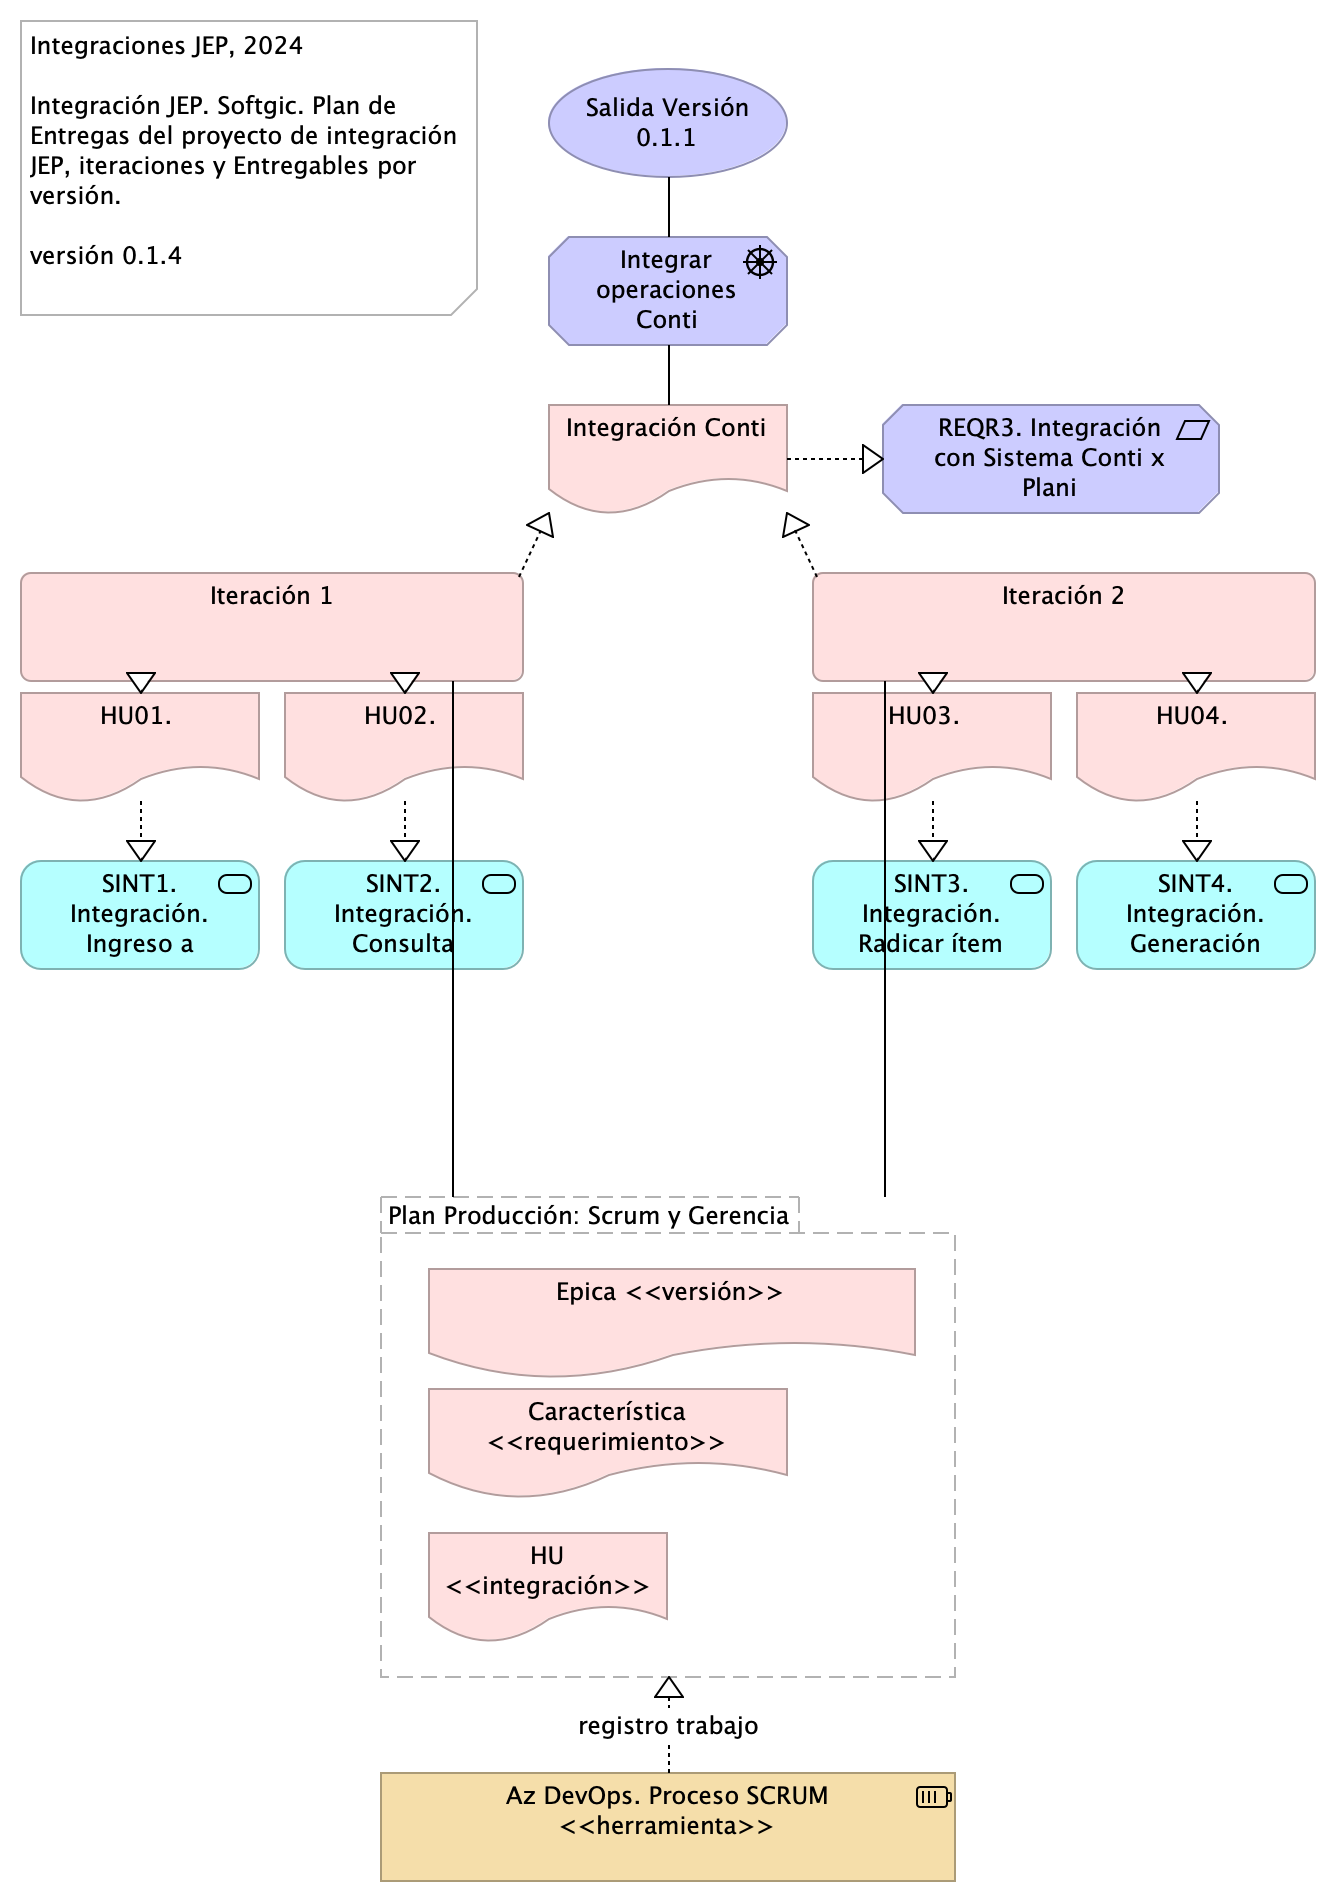
\includegraphics[width=\textwidth,height=5.20833in]{images/06.ENTRG.1n.1a.IntegraroperacionesConti.png}
\caption{06.ENTRG.1n.1a. Integrar operaciones Conti. \emph{Fuente:
Repositorio arquitectura Integración JEP
(2024)}}\label{fig:id-c31668d4d5dd44309f42fdd5fb2a7a53}
\end{figure}

\subsubsection{Catálogo de
Elementos}\label{sec:catuxe1logo-de-elementos-3}

\begin{longtable}[]{@{}
  >{\raggedright\arraybackslash}p{(\columnwidth - 4\tabcolsep) * \real{0.3000}}
  >{\raggedright\arraybackslash}p{(\columnwidth - 4\tabcolsep) * \real{0.2000}}
  >{\raggedright\arraybackslash}p{(\columnwidth - 4\tabcolsep) * \real{0.5000}}@{}}
\caption{\label{tbl:tblelement-06.ENTRG.1n.1a.IntegraroperacionesConti-id}Elementos
de la vista.}\tabularnewline
\toprule\noalign{}
\begin{minipage}[b]{\linewidth}\raggedright
Nombre
\end{minipage} & \begin{minipage}[b]{\linewidth}\raggedright
Tipo
\end{minipage} & \begin{minipage}[b]{\linewidth}\raggedright
Documentación
\end{minipage} \\
\midrule\noalign{}
\endfirsthead
\toprule\noalign{}
\begin{minipage}[b]{\linewidth}\raggedright
Nombre
\end{minipage} & \begin{minipage}[b]{\linewidth}\raggedright
Tipo
\end{minipage} & \begin{minipage}[b]{\linewidth}\raggedright
Documentación
\end{minipage} \\
\midrule\noalign{}
\endhead
\bottomrule\noalign{}
\endlastfoot
Integración Conti & Deliverable & Épica de entrega de la solución de
integración JEP, 2024, que contiene las iteraciones que realizarán la
característica `Integrar operaciones Conti'. \\
Integrar operaciones Conti & Driver & Característica de integración de
Conti contenido en la solución de integración JEP, 2024. \\
REQR3. Integración con Sistema Conti x Plani & Requirement & Atendiendo
la necesidad de la Subdirección de Contratación de implementar el flujo
de gestión precontractual en el sistema de Gestión Documental - Conti se
requiere contar con la información de los ítems del Plan Anual de
Adquisiciones -- PAA para iniciar el proceso, la cual se encuentra
gestionada en el Sistema de Gestión y Planeación Institucional PLANi. \\
SINT1. Integración. Ingreso a Conti & Application Service & Tareas de
desarrollo * Interoperabilidad IOP1. Transporte / Entrega Consulta
Negocio * Modelo de datos (XML, RBDMS, \ldots) * Esquema de datos (XSD,
DTD, JSON-E\ldots) * Contratos de interoperabilidad (WSDL, API\ldots) *
Mensajes petición IN (API, XML\ldots) * Mensajes respuesta OUT (API,
XML\ldots) * Mensajes excepción (API, XML\ldots) * Transporte (REST,
SOAP) * Función lógica (JEE, \ldots) * Registro y envío de actividad \\
SINT2. Integración. Consulta ítem de Conti & Application Service &
Tareas de desarrollo * Interoperabilidad IOP1. Transporte / Entrega
Consulta Negocio * Modelo de datos (XML, RBDMS, \ldots) * Esquema de
datos (XSD, DTD, JSON-E\ldots) * Contratos de interoperabilidad (WSDL,
API\ldots) * Mensajes petición IN (API, XML\ldots) * Mensajes respuesta
OUT (API, XML\ldots) * Mensajes excepción (API, XML\ldots) * Transporte
(REST, SOAP) * Función lógica (JEE, \ldots) * Registro y envío de
actividad \\
SINT3. Integración. Radicar ítem & Application Service & Tareas de
desarrollo * Interoperabilidad IOP1. Transporte / Entrega Consulta
Negocio * Modelo de datos (XML, RBDMS, \ldots) * Esquema de datos (XSD,
DTD, JSON-E\ldots) * Contratos de interoperabilidad (WSDL, API\ldots) *
Mensajes petición IN (API, XML\ldots) * Mensajes respuesta OUT (API,
XML\ldots) * Mensajes excepción (API, XML\ldots) * Transporte (REST,
SOAP) * Función lógica (JEE, \ldots) * Registro y envío de actividad \\
SINT4. Integración. Generación de documentos & Application Service &
Tareas de desarrollo * Interoperabilidad IOP1. Transporte / Entrega
Consulta Negocio * Modelo de datos (XML, RBDMS, \ldots) * Esquema de
datos (XSD, DTD, JSON-E\ldots) * Contratos de interoperabilidad (WSDL,
API\ldots) * Mensajes petición IN (API, XML\ldots) * Mensajes respuesta
OUT (API, XML\ldots) * Mensajes excepción (API, XML\ldots) * Transporte
(REST, SOAP) * Función lógica (JEE, \ldots) * Registro y envío de
actividad \\
\end{longtable}

\newpage

\section{Modelo de Despliegue de Requerimientos de Interoperabilidad
Proyecto
JEP}\label{sec:modelo-de-despliegue-de-requerimientos-de-interoperabilidad-proyecto-jep}

\subsection{Despliegue de Entregas de
Requerimientos}\label{sec:despliegue-de-entregas-de-requerimientos}

\begin{quote}
Integraciones JEP, 2024 Integración JEP. Softgic. Plan de Entregas del
proyecto de integración y despliegue JEP, iteraciones y Entregables por
versión. versión 0.1.14
\end{quote}

Los servicios implementados contenidos en los requerimientos se pueden
desplegar sobre la red de unidades de despliegue (pods) dispuesta por la
JEP y acordada con el contratista.

En esta organización propuesta, los servicios de integración
implementados pueden ser desplegados en uno, o varios contenedores, y en
unidades de despliegue (pods) distintas.

\begin{figure}
\centering
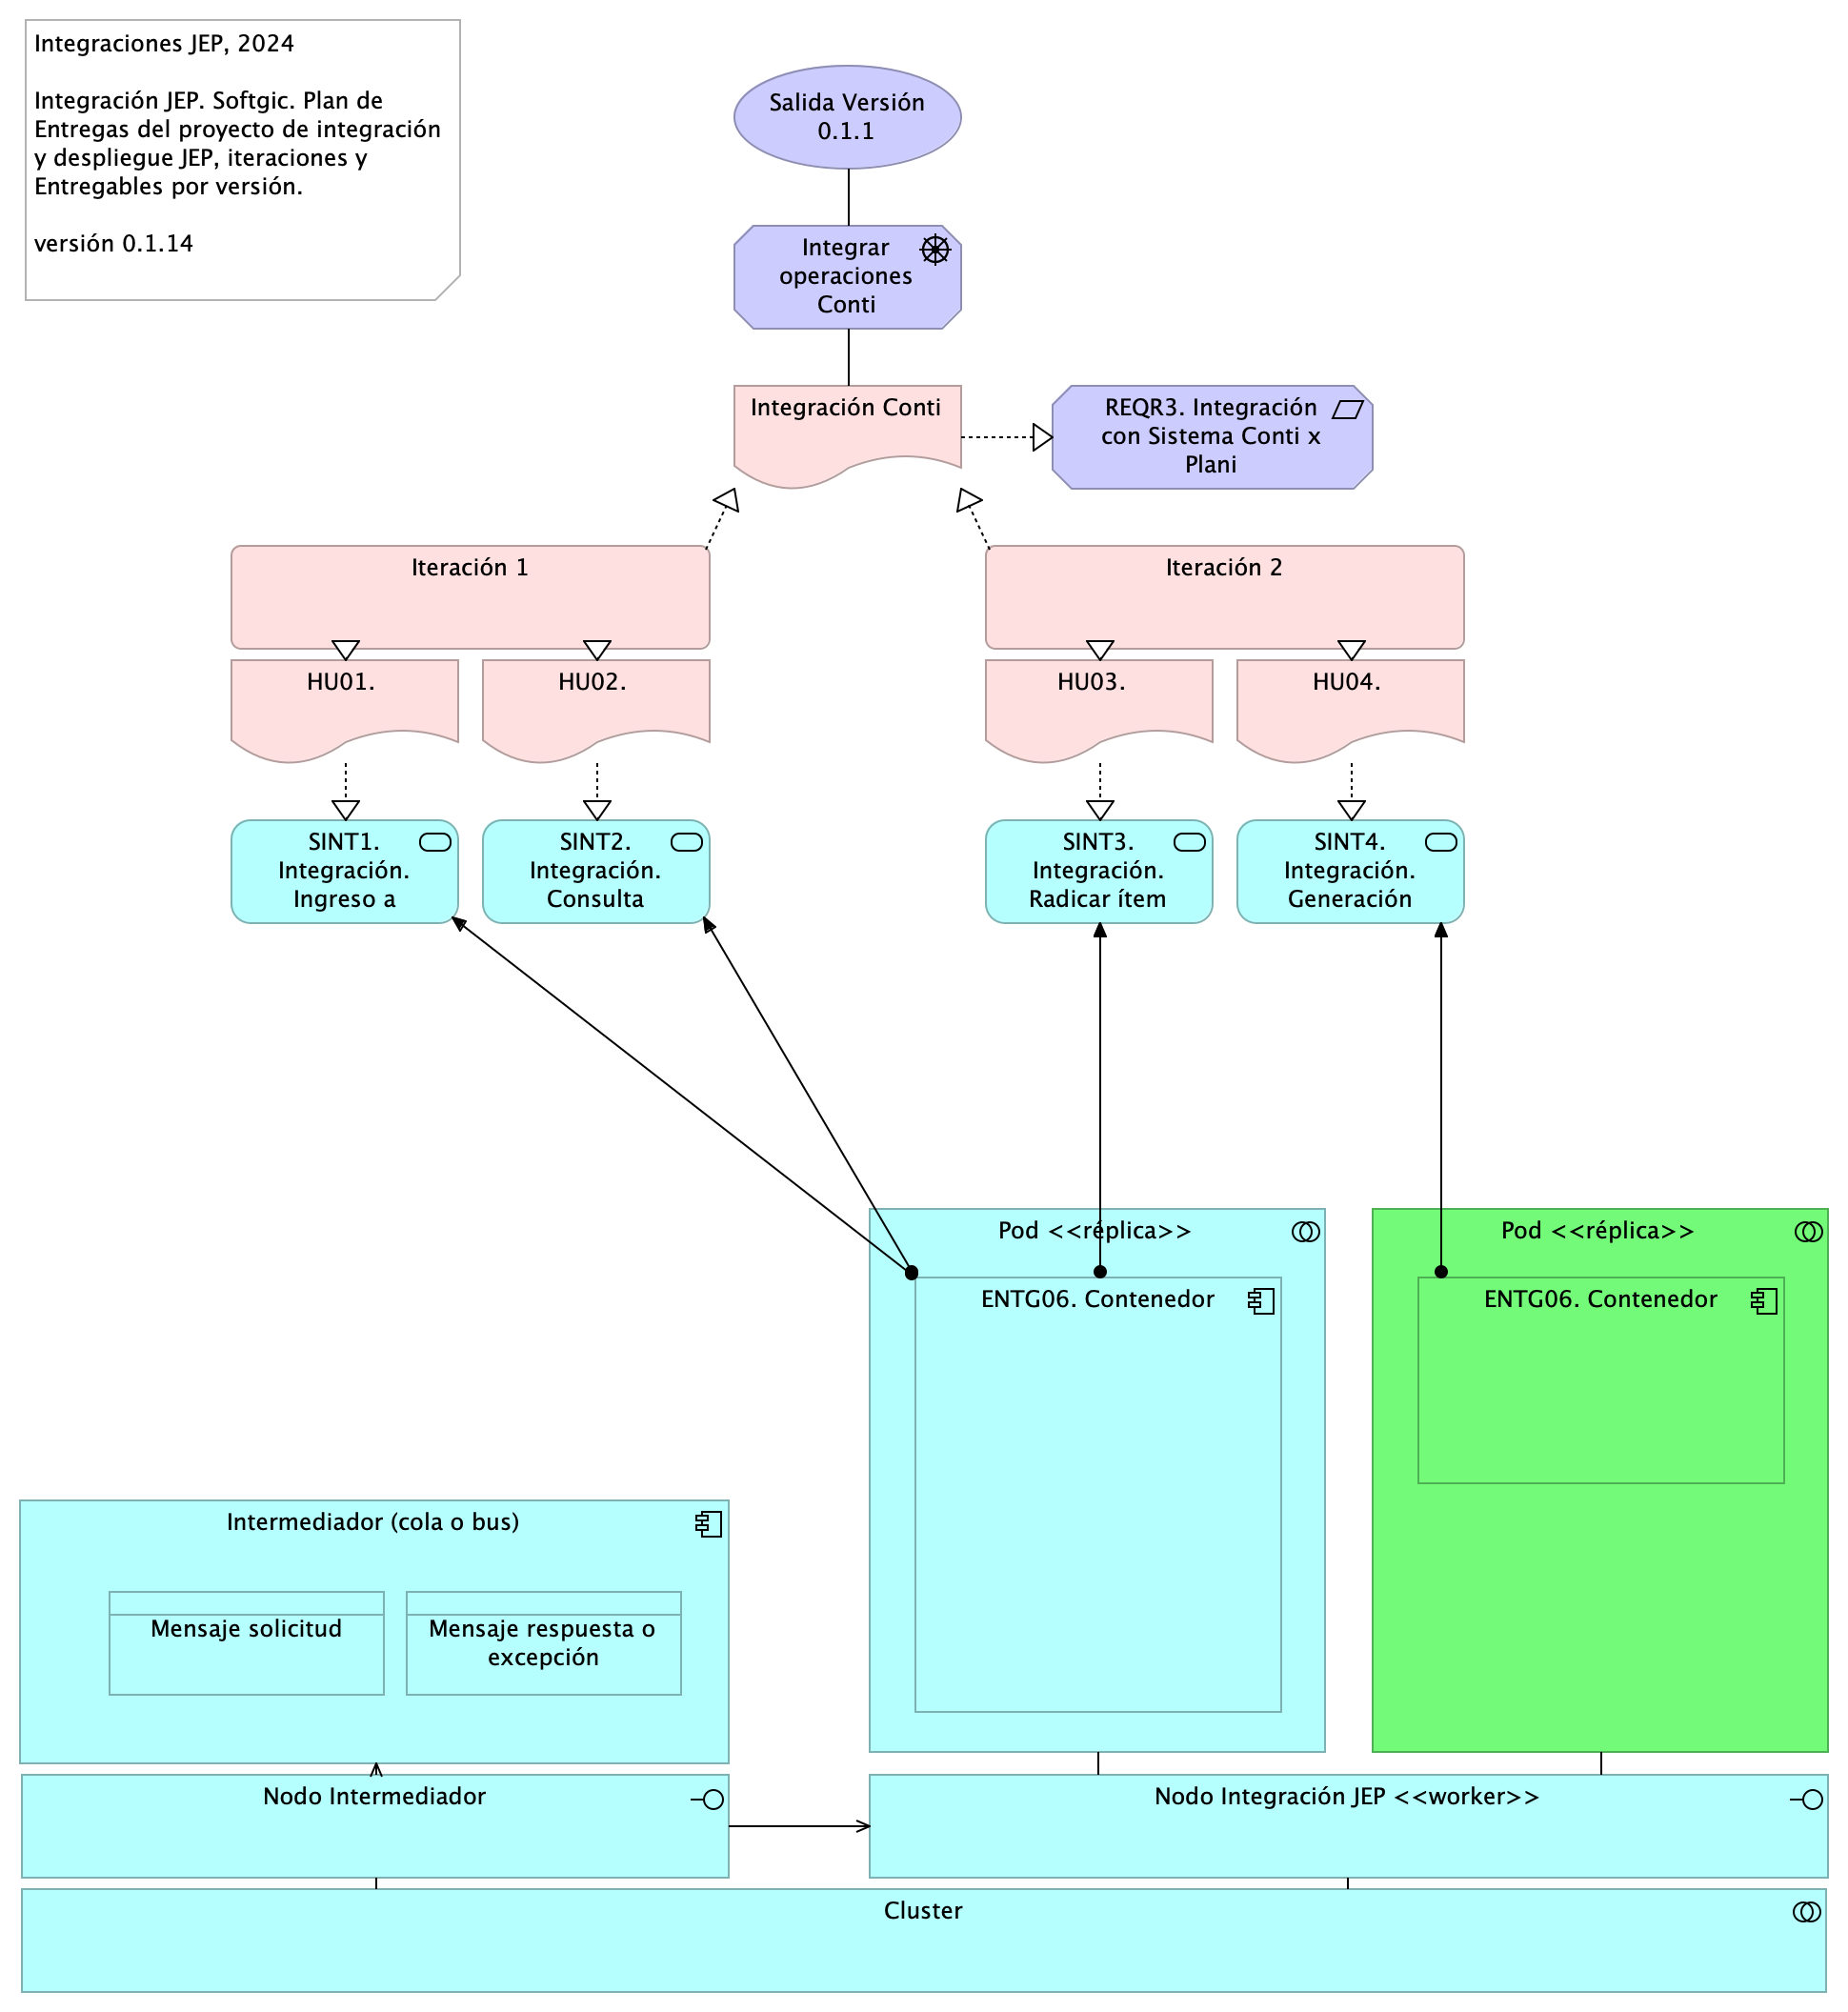
\includegraphics[width=\textwidth,height=5.20833in]{images/06.ENTRG.1n.1a.1.Despliegue.png}
\caption{06.ENTRG.1n.1a.1. Despliegue. \emph{Fuente: Repositorio
arquitectura Integración JEP
(2024)}}\label{fig:id-203e737545e449e59334b47d3034d956}
\end{figure}

\subsubsection{Catálogo de
Elementos}\label{sec:catuxe1logo-de-elementos-4}

\begin{longtable}[]{@{}
  >{\raggedright\arraybackslash}p{(\columnwidth - 4\tabcolsep) * \real{0.3000}}
  >{\raggedright\arraybackslash}p{(\columnwidth - 4\tabcolsep) * \real{0.2000}}
  >{\raggedright\arraybackslash}p{(\columnwidth - 4\tabcolsep) * \real{0.5000}}@{}}
\caption{\label{tbl:tblelement-06.ENTRG.1n.1a.1.Despliegue-id}Elementos
de la vista.}\tabularnewline
\toprule\noalign{}
\begin{minipage}[b]{\linewidth}\raggedright
Nombre
\end{minipage} & \begin{minipage}[b]{\linewidth}\raggedright
Tipo
\end{minipage} & \begin{minipage}[b]{\linewidth}\raggedright
Documentación
\end{minipage} \\
\midrule\noalign{}
\endfirsthead
\toprule\noalign{}
\begin{minipage}[b]{\linewidth}\raggedright
Nombre
\end{minipage} & \begin{minipage}[b]{\linewidth}\raggedright
Tipo
\end{minipage} & \begin{minipage}[b]{\linewidth}\raggedright
Documentación
\end{minipage} \\
\midrule\noalign{}
\endhead
\bottomrule\noalign{}
\endlastfoot
Cluster & Application Collaboration & Orquestador de nodos y servicios
(contendores) de la JEP. \\
ENTG06. Contenedor & Application Component & Contenedores de los
servicios de integración del proyecto desplegados en la infraestructura
tecnológica JEP. \\
Integración Conti & Deliverable & Épica de entrega de la solución de
integración JEP, 2024, que contiene las iteraciones que realizarán la
característica `Integrar operaciones Conti'. \\
Integrar operaciones Conti & Driver & Característica de integración de
Conti contenido en la solución de integración JEP, 2024. \\
Intermediador (cola o bus) & Application Component & Bus de Red Hat,
aplicación cliente Quarkus, o intermediador de integración Apache
Camel. \\
Mensaje respuesta o excepción & Data Object & Formato predefinido de
intercambio de datos. \\
Mensaje solicitud & Data Object & Formato predefinido de intercambio de
datos. \\
Nodo Integración JEP (worker) & Application Interface & Nodo lógico en
donde corren los contenedores. \\
Nodo Intermediador & Application Interface & Nodo lógico en donde corren
los contenedores. \\
REQR3. Integración con Sistema Conti x Plani & Requirement & Atendiendo
la necesidad de la Subdirección de Contratación de implementar el flujo
de gestión precontractual en el sistema de Gestión Documental - Conti se
requiere contar con la información de los ítems del Plan Anual de
Adquisiciones -- PAA para iniciar el proceso, la cual se encuentra
gestionada en el Sistema de Gestión y Planeación Institucional PLANi. \\
SINT1. Integración. Ingreso a Conti & Application Service & Tareas de
desarrollo * Interoperabilidad IOP1. Transporte / Entrega Consulta
Negocio * Modelo de datos (XML, RBDMS, \ldots) * Esquema de datos (XSD,
DTD, JSON-E\ldots) * Contratos de interoperabilidad (WSDL, API\ldots) *
Mensajes petición IN (API, XML\ldots) * Mensajes respuesta OUT (API,
XML\ldots) * Mensajes excepción (API, XML\ldots) * Transporte (REST,
SOAP) * Función lógica (JEE, \ldots) * Registro y envío de actividad \\
SINT2. Integración. Consulta ítem de Conti & Application Service &
Tareas de desarrollo * Interoperabilidad IOP1. Transporte / Entrega
Consulta Negocio * Modelo de datos (XML, RBDMS, \ldots) * Esquema de
datos (XSD, DTD, JSON-E\ldots) * Contratos de interoperabilidad (WSDL,
API\ldots) * Mensajes petición IN (API, XML\ldots) * Mensajes respuesta
OUT (API, XML\ldots) * Mensajes excepción (API, XML\ldots) * Transporte
(REST, SOAP) * Función lógica (JEE, \ldots) * Registro y envío de
actividad \\
SINT3. Integración. Radicar ítem & Application Service & Tareas de
desarrollo * Interoperabilidad IOP1. Transporte / Entrega Consulta
Negocio * Modelo de datos (XML, RBDMS, \ldots) * Esquema de datos (XSD,
DTD, JSON-E\ldots) * Contratos de interoperabilidad (WSDL, API\ldots) *
Mensajes petición IN (API, XML\ldots) * Mensajes respuesta OUT (API,
XML\ldots) * Mensajes excepción (API, XML\ldots) * Transporte (REST,
SOAP) * Función lógica (JEE, \ldots) * Registro y envío de actividad \\
SINT4. Integración. Generación de documentos & Application Service &
Tareas de desarrollo * Interoperabilidad IOP1. Transporte / Entrega
Consulta Negocio * Modelo de datos (XML, RBDMS, \ldots) * Esquema de
datos (XSD, DTD, JSON-E\ldots) * Contratos de interoperabilidad (WSDL,
API\ldots) * Mensajes petición IN (API, XML\ldots) * Mensajes respuesta
OUT (API, XML\ldots) * Mensajes excepción (API, XML\ldots) * Transporte
(REST, SOAP) * Función lógica (JEE, \ldots) * Registro y envío de
actividad \\
\end{longtable}

\end{document}
